% Requires: \usepackage{graphicx,tikz}
% Image paths are relative to this .tex file's location.
% Generated by: smixae latex figures  (experiment: gemma_2_9b_l20)

\begin{figure*}[t]
\centering
\noindent\makebox[\linewidth][c]{%
\begin{minipage}[t]{0.3949\linewidth}%
\vspace{0pt}\centering%
\begin{minipage}[c][4.0cm][c]{0.7407\linewidth}%
\centering%
\begin{tikzpicture}[baseline=(img.base)]
  \node[inner sep=0pt] (img) {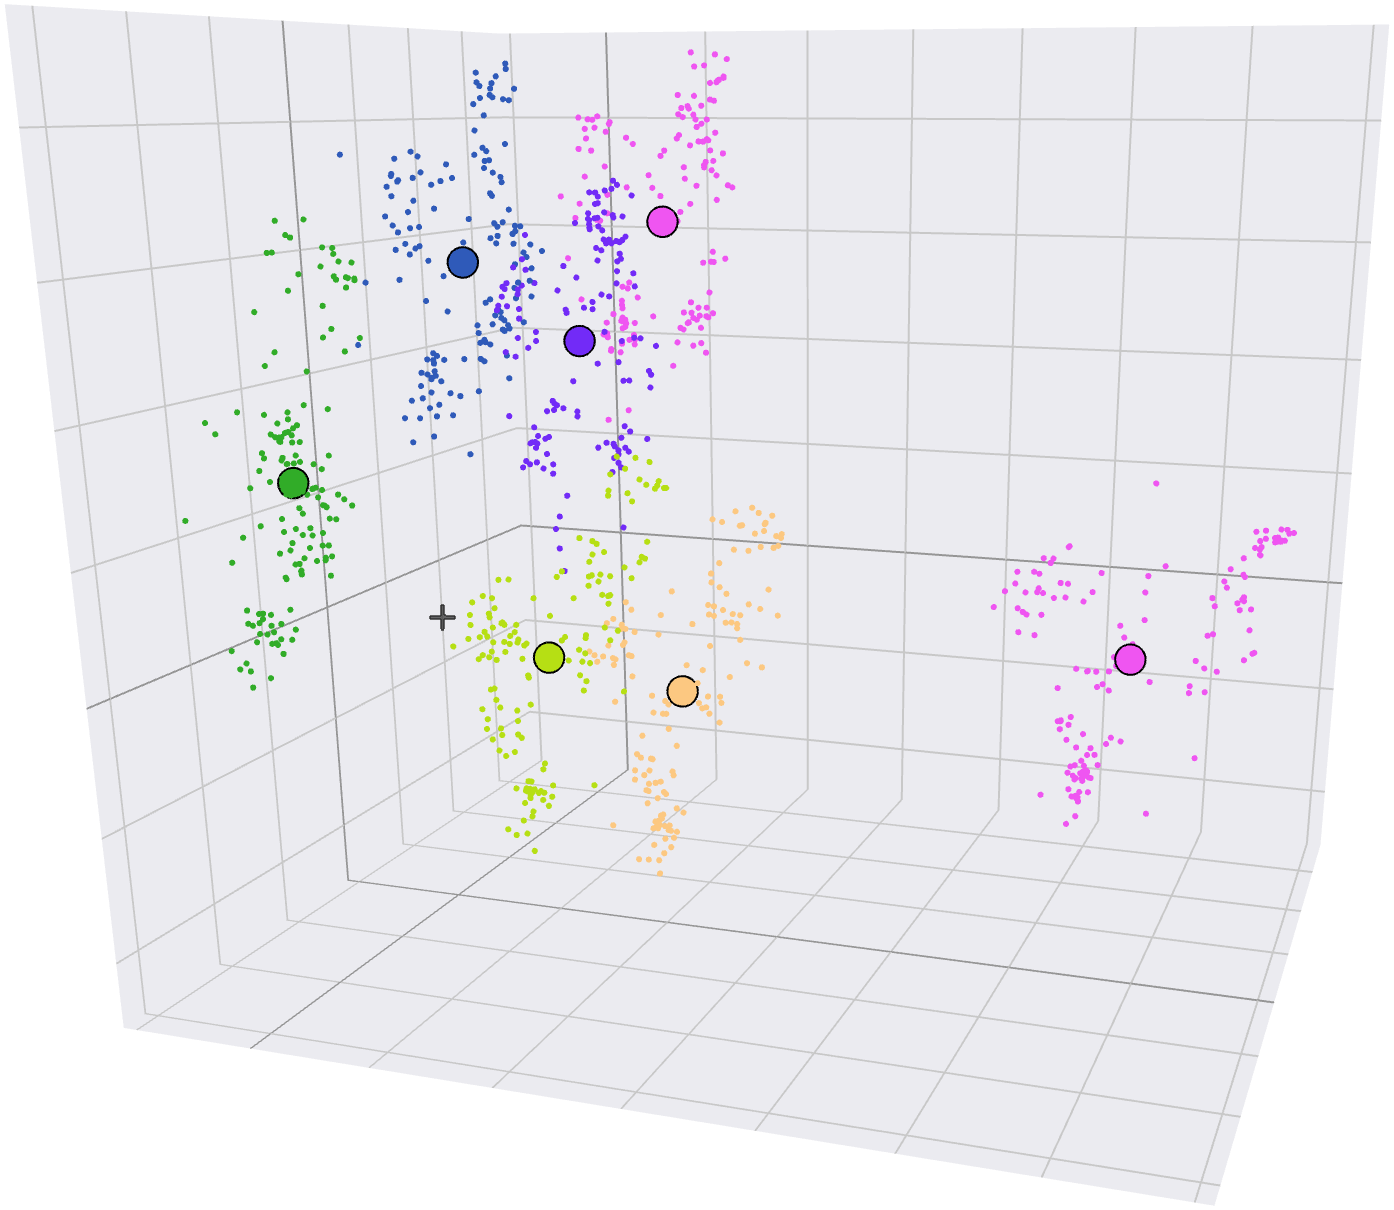
\includegraphics[width=\linewidth,height=4.0cm,keepaspectratio]{paper/camera_ready/gemma_2_9b_l20__weekdays_—_expert_analysis__E1808__cyc_7d__r2__0.7594__scatter.png}};
  \node[anchor=north west, inner sep=2pt, overlay] at (img.north west) {\small\textbf{(a)}};
\end{tikzpicture}%
\end{minipage}%
\begin{minipage}[c][4.0cm][c]{0.2593\linewidth}%
\centering%

\includegraphics[width=\linewidth,height=4.0cm,keepaspectratio]{paper/legends/legend_weekdays.png}%
\end{minipage}%
\par\vspace{1pt}%
{\footnotesize\textit{Weekdays}}%
\end{minipage}%
}
\vspace{5pt}

\noindent\makebox[\linewidth][c]{%
\begin{minipage}[t]{0.9800\linewidth}%
\vspace{0pt}\centering%
\begin{minipage}[c][4.0cm][c]{0.2985\linewidth}%
\centering%
\begin{tikzpicture}[baseline=(img.base)]
  \node[inner sep=0pt] (img) {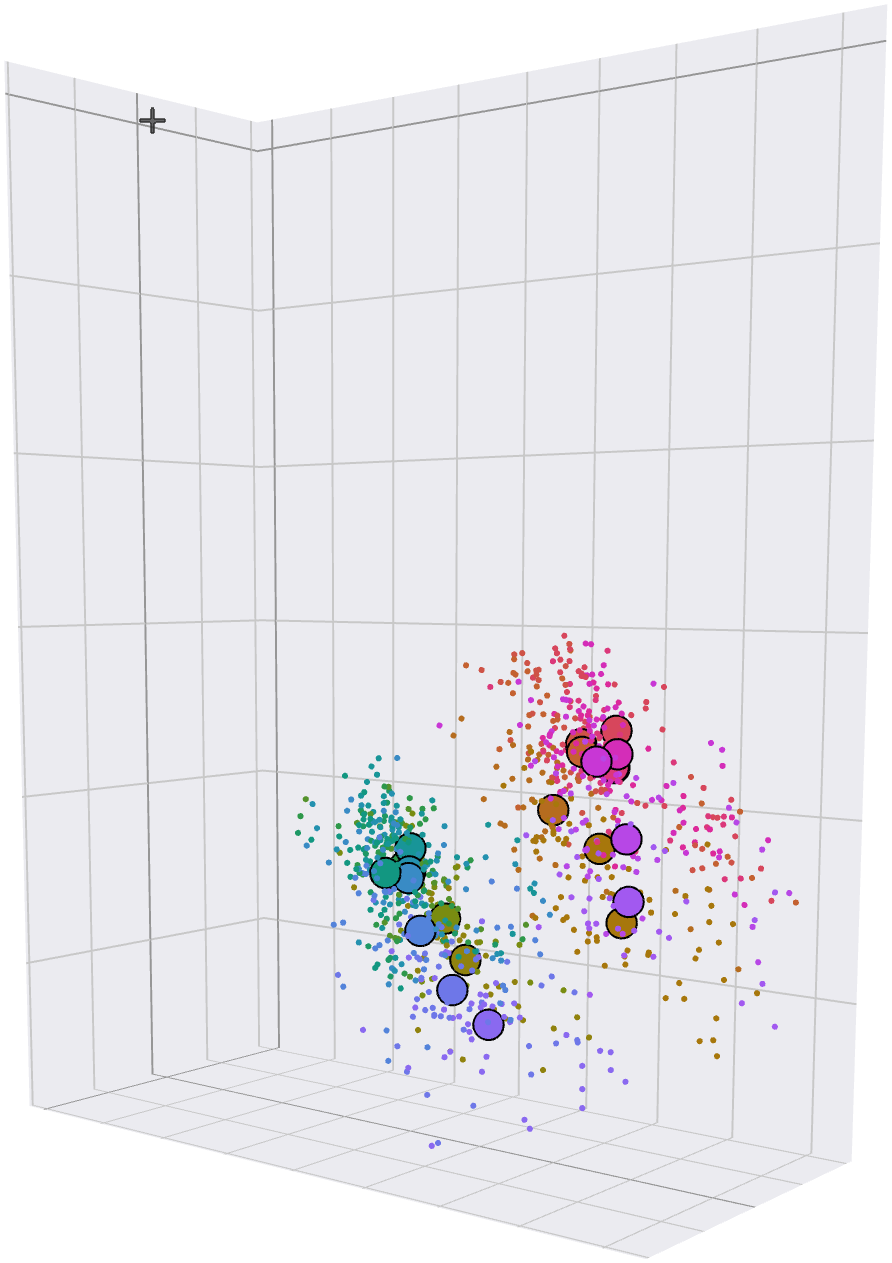
\includegraphics[width=\linewidth,height=4.0cm,keepaspectratio]{paper/camera_ready/gemma_2_9b_l20__hours_—_expert_analysis__E1041__am_pm__acc__0.9969__scatter.png}};
  \node[anchor=north west, inner sep=2pt, overlay] at (img.north west) {\small\textbf{(b)}};
\end{tikzpicture}%
\end{minipage}%
\begin{minipage}[c][4.0cm][c]{0.2985\linewidth}%
\centering%
\begin{tikzpicture}[baseline=(img.base)]
  \node[inner sep=0pt] (img) {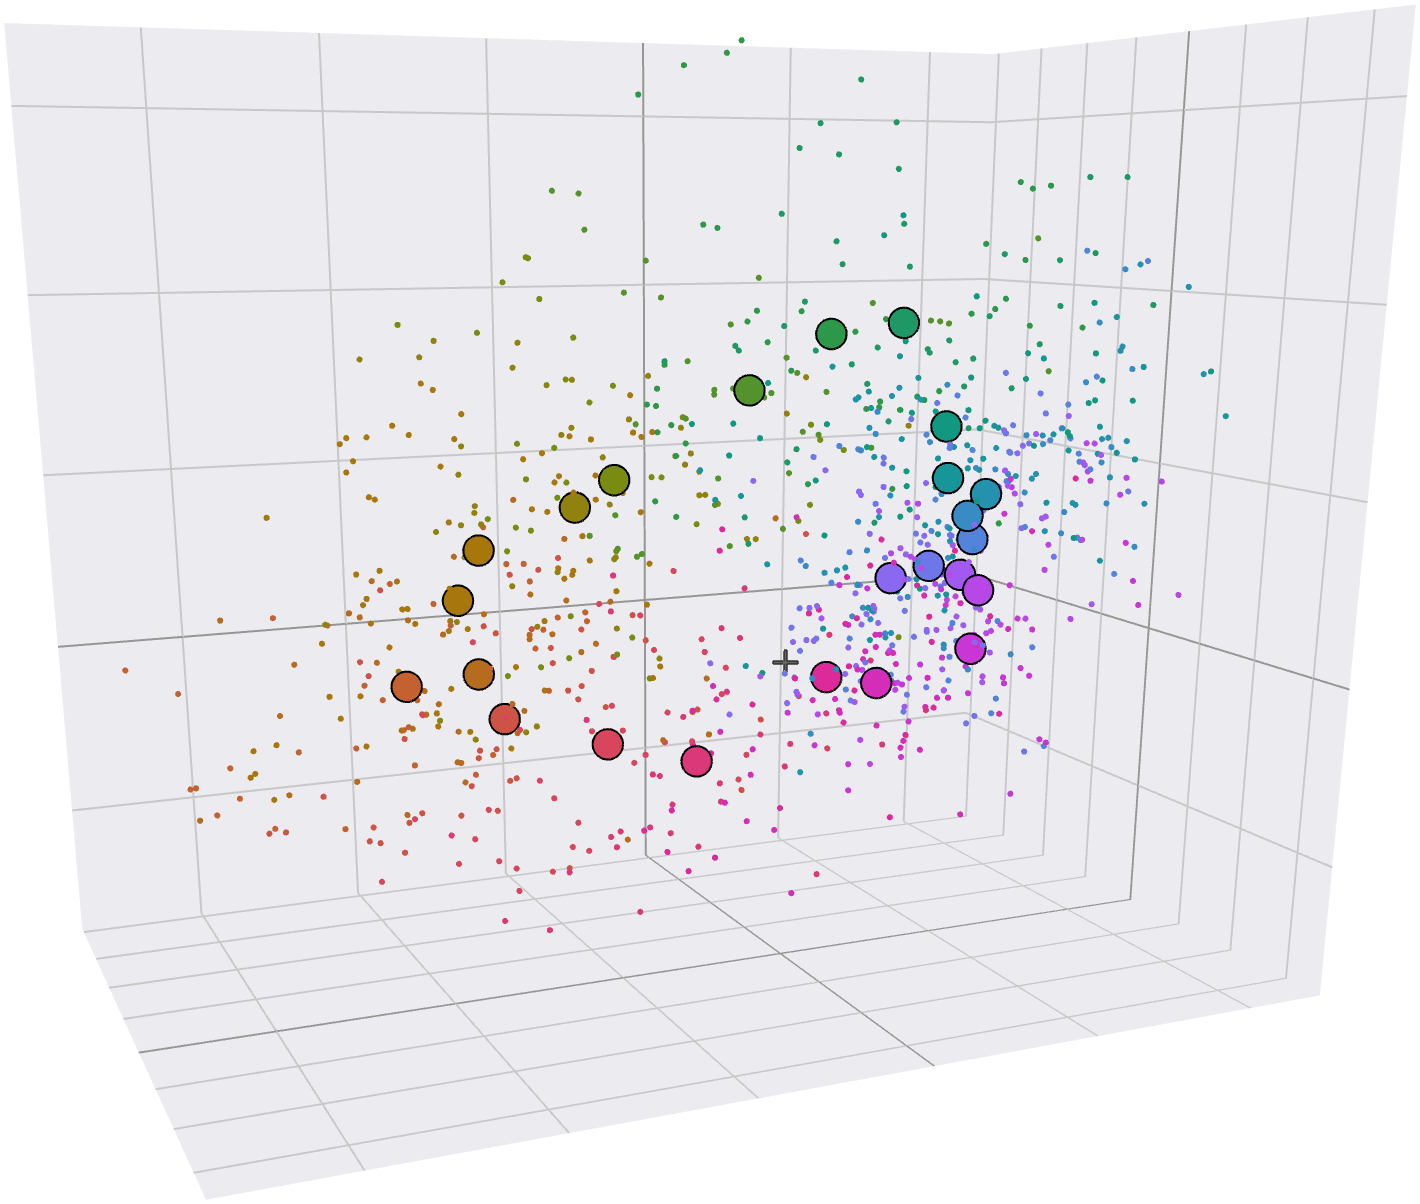
\includegraphics[width=\linewidth,height=4.0cm,keepaspectratio]{paper/camera_ready/gemma_2_9b_l20__hours_—_expert_analysis__E1701__cyc_24h__r2__0.6186__scatter.png}};
  \node[anchor=north west, inner sep=2pt, overlay] at (img.north west) {\small\textbf{(c)}};
\end{tikzpicture}%
\end{minipage}%
\begin{minipage}[c][4.0cm][c]{0.2985\linewidth}%
\centering%
\begin{tikzpicture}[baseline=(img.base)]
  \node[inner sep=0pt] (img) {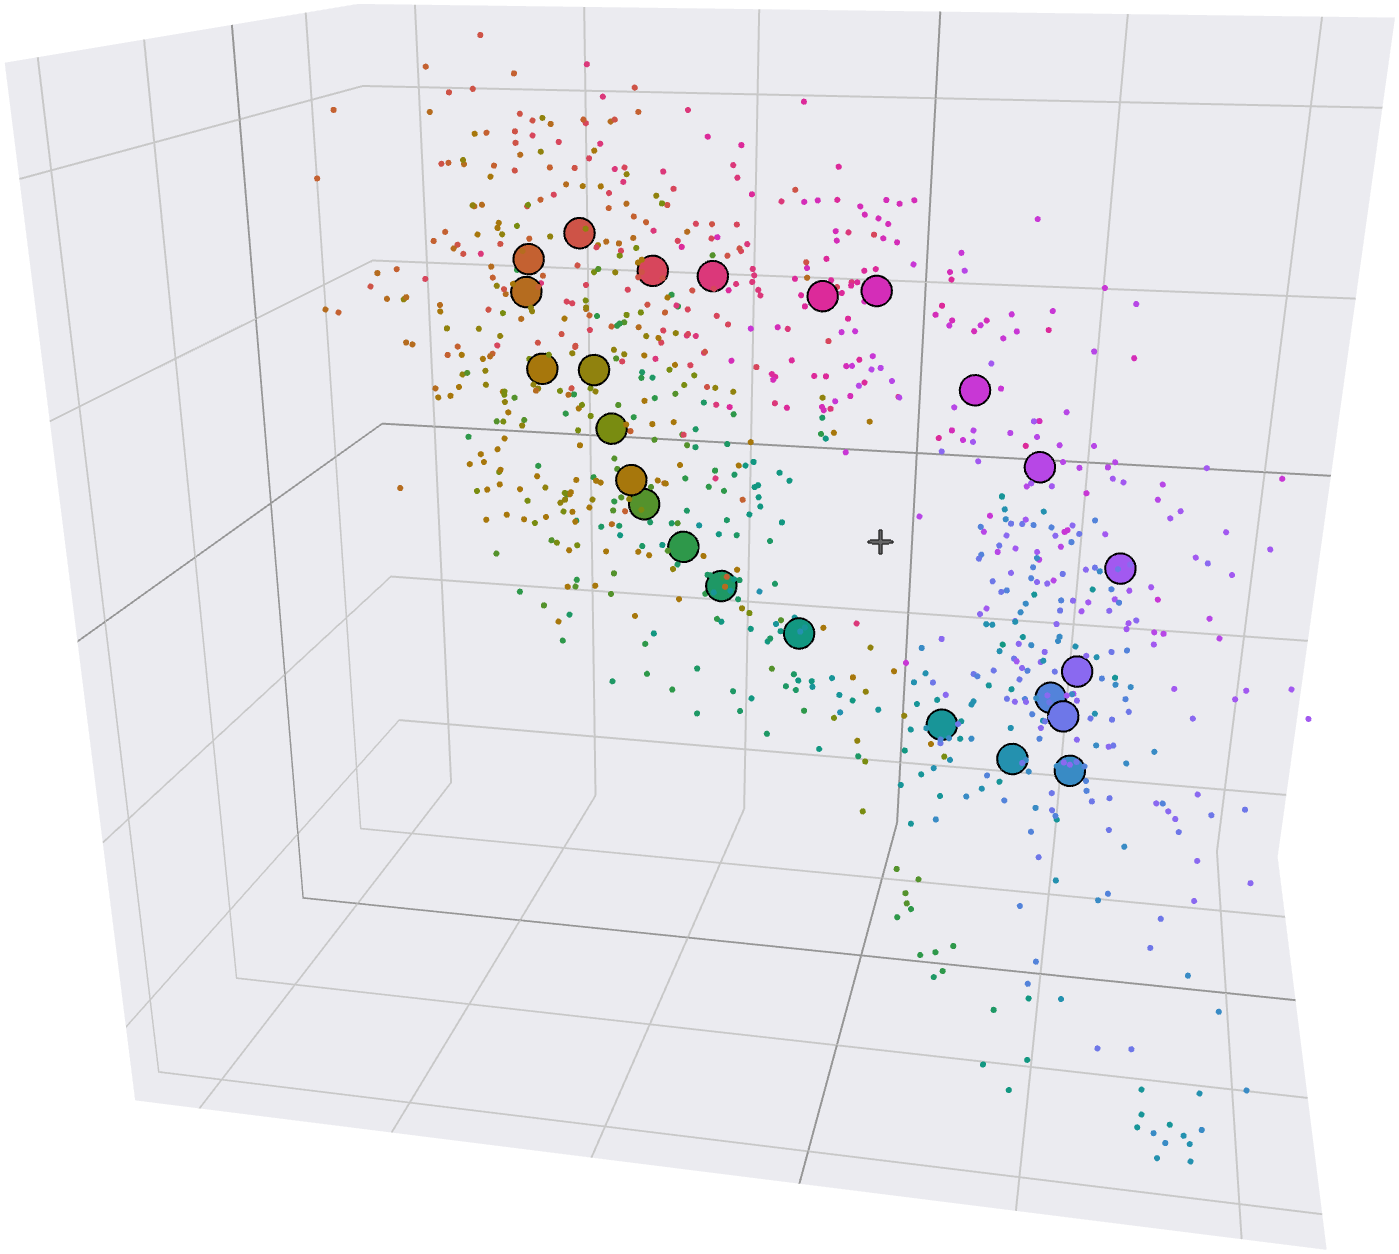
\includegraphics[width=\linewidth,height=4.0cm,keepaspectratio]{paper/camera_ready/gemma_2_9b_l20__hours_—_expert_analysis__E691__cyc_24h__r2__0.6322__scatter.png}};
  \node[anchor=north west, inner sep=2pt, overlay] at (img.north west) {\small\textbf{(d)}};
\end{tikzpicture}%
\end{minipage}%
\begin{minipage}[c][4.0cm][c]{0.1045\linewidth}%
\centering%

\includegraphics[width=\linewidth,height=4.0cm,keepaspectratio]{paper/legends/legend_hours.png}%
\end{minipage}%
\par\vspace{1pt}%
{\footnotesize\textit{Hours}}%
\end{minipage}%
}
\vspace{5pt}

\noindent\makebox[\linewidth][c]{%
\begin{minipage}[t]{0.3267\linewidth}%
\vspace{0pt}\centering%
\begin{minipage}[c][4.0cm][c]{0.7407\linewidth}%
\centering%
\begin{tikzpicture}[baseline=(img.base)]
  \node[inner sep=0pt] (img) {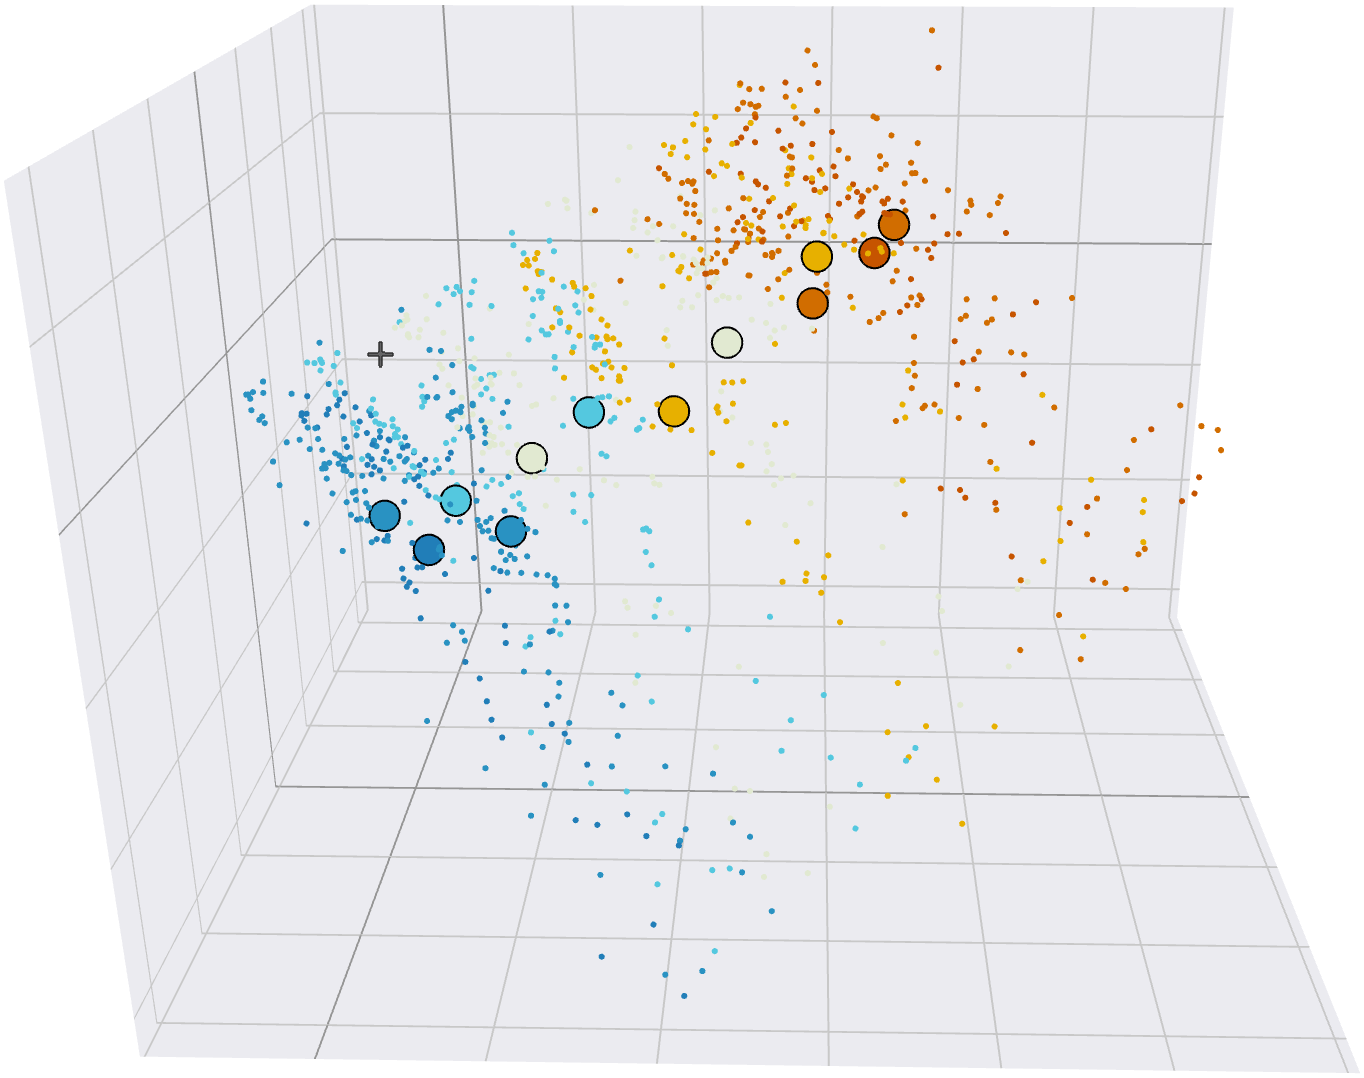
\includegraphics[width=\linewidth,height=4.0cm,keepaspectratio]{paper/camera_ready/gemma_2_9b_l20__months_—_expert_analysis__E1628__cyc_12m__r2__0.4700__scatter.png}};
  \node[anchor=north west, inner sep=2pt, overlay] at (img.north west) {\small\textbf{(e)}};
\end{tikzpicture}%
\end{minipage}%
\begin{minipage}[c][4.0cm][c]{0.2593\linewidth}%
\centering%

\includegraphics[width=\linewidth,height=4.0cm,keepaspectratio]{paper/legends/legend_months.png}%
\end{minipage}%
\par\vspace{1pt}%
{\footnotesize\textit{Months}}%
\end{minipage}%
\hspace{2.5mm}%
\begin{minipage}[t]{0.3267\linewidth}%
\vspace{0pt}\centering%
\begin{minipage}[c][4.0cm][c]{0.7407\linewidth}%
\centering%
\begin{tikzpicture}[baseline=(img.base)]
  \node[inner sep=0pt] (img) {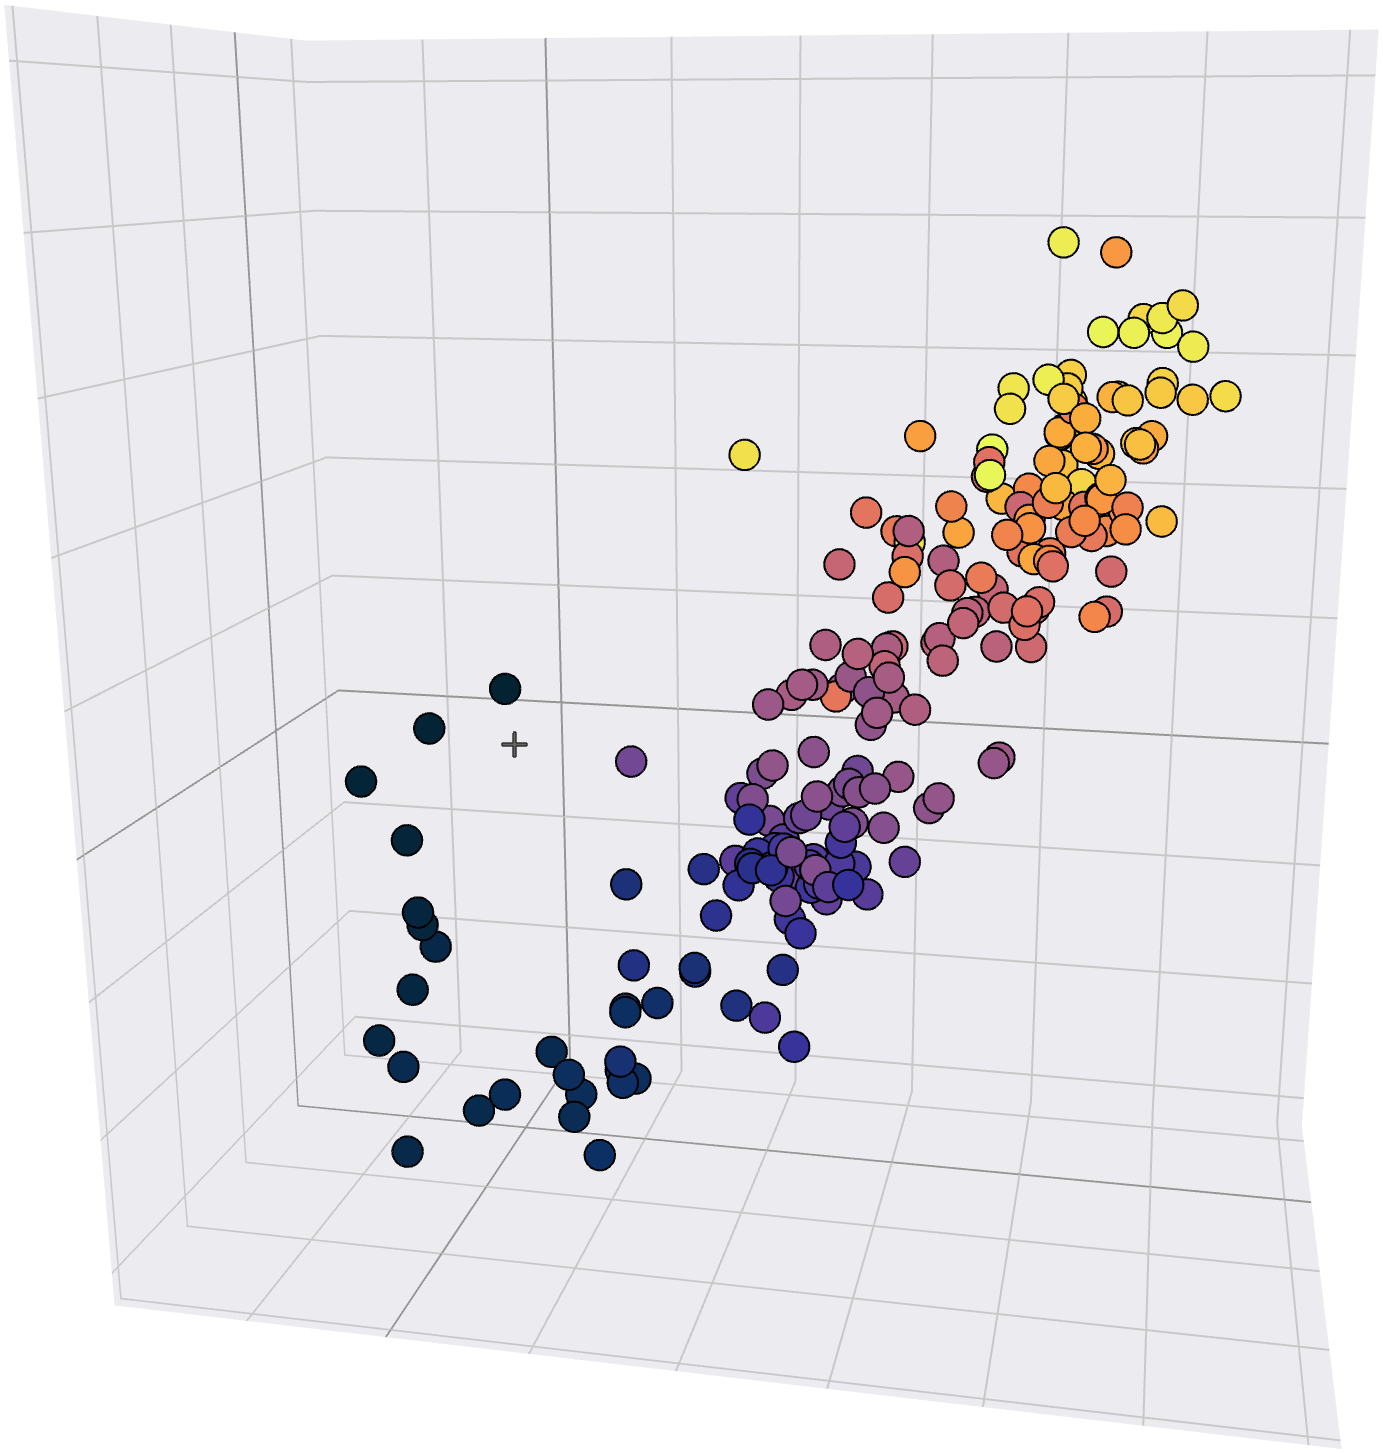
\includegraphics[width=\linewidth,height=4.0cm,keepaspectratio]{paper/camera_ready/gemma_2_9b_l20__temperatures_—_expert_analysis__E1716__linear_f__r2__0.8101__means.png}};
  \node[anchor=north west, inner sep=2pt, overlay] at (img.north west) {\small\textbf{(f)}};
\end{tikzpicture}%
\end{minipage}%
\begin{minipage}[c][4.0cm][c]{0.2593\linewidth}%
\centering%

\includegraphics[width=\linewidth,height=4.0cm,keepaspectratio]{paper/legends/legend_temperatures.png}%
\end{minipage}%
\par\vspace{1pt}%
{\footnotesize\textit{Temperature}}%
\end{minipage}%
\hspace{2.5mm}%
\begin{minipage}[t]{0.3267\linewidth}%
\vspace{0pt}\centering%
\begin{minipage}[c][4.0cm][c]{0.7407\linewidth}%
\centering%
\begin{tikzpicture}[baseline=(img.base)]
  \node[inner sep=0pt] (img) {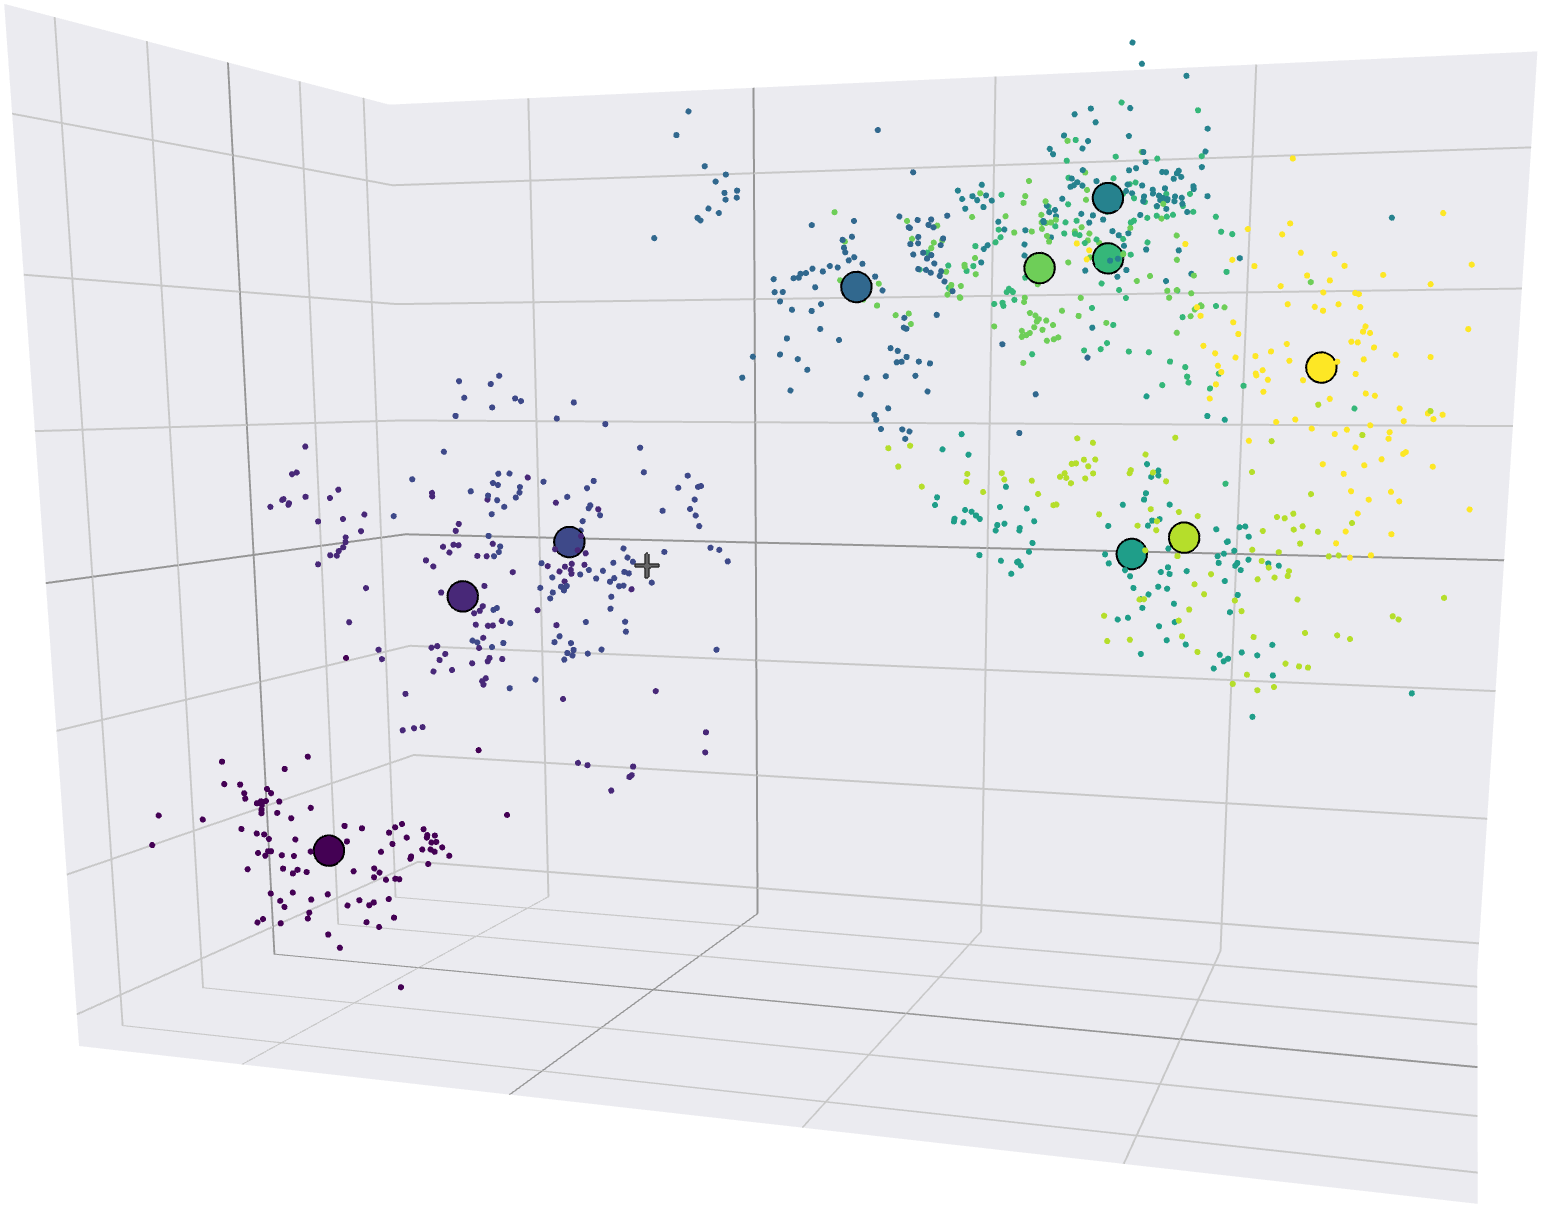
\includegraphics[width=\linewidth,height=4.0cm,keepaspectratio]{paper/camera_ready/gemma_2_9b_l20__time_units_—_expert_analysis__E923__log_duration__r2__0.8571__scatter.png}};
  \node[anchor=north west, inner sep=2pt, overlay] at (img.north west) {\small\textbf{(g)}};
\end{tikzpicture}%
\end{minipage}%
\begin{minipage}[c][4.0cm][c]{0.2593\linewidth}%
\centering%

\includegraphics[width=\linewidth,height=4.0cm,keepaspectratio]{paper/legends/legend_time_units.png}%
\end{minipage}%
\par\vspace{1pt}%
{\footnotesize\textit{Time Units}}%
\end{minipage}%
}
\caption{Gemma 2 9B, Layer 20. \textbf{Weekdays}: (a) Expert 1808, 7-Day Ring ($R^2$\,=\,0.759).  \textbf{Hours}: (b) Expert 1041, AM vs PM (Accuracy\,=\,0.997). (c) Expert 1701, 24-Hour Ring ($R^2$\,=\,0.619). (d) Expert 691, 24-Hour Ring ($R^2$\,=\,0.632).  \textbf{Months}: (e) Expert 1628, 12-Month Ring ($R^2$\,=\,0.470).  \textbf{Temperature}: (f) Expert 1716, Linear \textdegree F ($R^2$\,=\,0.810).  \textbf{Time Units}: (g) Expert 923, log Duration ($R^2$\,=\,0.857). Larger points denote class mean activations in the bottleneck space; smaller points are individual token activations.}
\end{figure*}
